\documentclass[main.tex]{subfiles}
\pagenumbering{arabic}
\newcommand\chapterlabel{units}

\begin{document}
\linenumbers



\chapter[Measurements]{Measurements}
\label{ch:measurements}
 \begin{marginfigure}
\begin{tikzpicture} \node (a) at (0,0) {\includegraphics[width=4cm]{chapter1/figure1}} node[rotate=90, font=\tiny] at ([yshift=.5cm,xshift=.1cm]a.south east) {\textsuperscript{\textcopyright} PngImg} ;
\end{tikzpicture}
\label{fig:marginfig}
\end{marginfigure}
\lettrine[lines=4]{\color{black!45}M}{easuring} is an important part of our everyday lives, and very probably you took several measurements today. You might now be sipping a cup of coffee, or perhaps you checked the outside temperature on a street thermometer. You might be planning to bake a cake and need to use a scale and a cup to measure the flour and sugar. A cup, a thermometer, or a scale are measuring devices. This chapter will cover how to accurately measure properties and, more importantly, how to transform measurements using prefixes and unit conversions. In this chapter, by learning how to measure and perform operations with units, you will gain experience performing basic chemistry calculations.
\begin{marginfigure}%LEARNING GOALS BOX
\begin{mytcbox}{GOALS}
\begin{enumerate}[label=\protect\circled{\color{white}\arabic*}]
\item Identify units and prefixes
\item Introduce/eliminate prefixes
\item Switch prefixes
\item Calculate significant figures
\item Carry out density calculations
\end{enumerate}
\end{mytcbox}
\vspace{1cm}
\begin{tcolorbox}[enhanced,colback=red!5!white,colframe=black!50!red,boxrule=1pt,
  arc=0pt,outer arc=0pt,drop heavy lifted shadow]
\faGears\ 
\docenvdef{Discussion:} (a) Discuss why is chemistry important for your career objective by listing three reasons that links chemistry with your career objective, (b) You have a glass filled with water and ice to its rim. If the ice melts will the water overflow the glass? Explain your reasoning. \end{tcolorbox}
\end{marginfigure}%LEARNING GOALS BOX





\section{Units of Measurements and systems of units}

You probably heard the term liter, kilogram or meter. These are units of measurement. Units can be classified into different \emph{systems of units}. For example, the unit \emph{meter} belongs to a different system than the unit \emph{mile}. In particular here we will address two main systems: the English System used in the US and the Metric System used by most of the industrialized world.
The \emph{Metric System} (MS) is used by  scientists throughout the world and is the most common measuring system based on the meter. The \emph{International System of Units} (SI) adopted the metric system in 1960 in order to provide additional uniformity for units used the sciences. This chapter will be mostly based on the SI units. In the following we will introduce some common units.

\sloppy
\begin{description}
\item[\docfilehook{Length}{Length}] What is your height? Length refers to distance and  both the metric and SI unit of length is the meter (m). A smaller unit of length would be the centimeter (cm) that is  commonly used in chemistry. The most important units of length are: meter, inch and mile.
  
\item[\docfilehook{Volume}{Volume}] How much milk do you usually buy? Maybe a gallon. Volume is the amount of space that a substance occupies. A liter (L) is commonly used to measure volume. The milliliter (mL) is more convenient for measuring smaller volumes of fluids in hospitals and laboratories. Gallon is still used in every-day life.  L, mL and gallon are units of volume. Units of volume are in general cubic units, so for example one liter is the same as one $dm^3$. We will cover cubit units further in this chapter.

\item[\docfilehook{Mass}{Mass}]What is you weight? The mass of an object is a measure of the quantity of material it contains. You may be more familiar with the term weight than with mass. However, mass and weight are not exactly the same, as  weight is a measure of the gravitational pull on an object. It differs depending on your location in the earth--in particular the height of your location. In the metric system, the unit for mass is the gram (g). The SI unit of mass, the kilogram (kg), is used for larger masses such as body weight. Pound, lb, is another unit of mass. The most important units of mass are: g, kg and lb.

\item[\docfilehook{Temperature}{Temperature}] How is the weather today? Is it cold or hot? You use a thermometer to measure temperature and for example assess how hot an object is, or how cold it is outside, or perhaps to determine if you have a fever.  Temperature tells us how hot or cold an object is. Temperature can be measured in numerous units such as Celsius ($^{\circ}$C), Fahrenheit ($^{\circ}$F), or kelvins (K). 

\item[\docfilehook{Time}{Time}]How long is your commute to from home work? It might take you hours to go to work, or maybe minutes. You probably think of time as years, days, minutes, or seconds. Of all these units, the International System of units (SI, abbreviated from the French Systeme international) uses seconds (s) to measure time. Still, time can be measured in s, min, or h and during this chapter we will learn how to convert units of time.

\end{description}
 
   \begin{marginfigure}[0cm]
   \begin{tikzpicture} \node (a) at (0,0) {\includegraphics[width=4cm, height=4cm]{chapter1/figure1-1}} node[rotate=90, font=\tiny] at ([yshift=.5cm,xshift=.1cm]a.south east) {\textsuperscript{\textcopyright} www.wallpaperflare.com} ;
\node[text width=5cm] at ([yshift=0.2cm]a.north) {\mytriangle{red}Scales measure mass};
\end{tikzpicture}
\begin{tikzpicture} \node (a) at (0,0) {\includegraphics[width=4cm, height=4cm]{chapter1/figure1-2}} node[rotate=90, font=\tiny] at ([yshift=.5cm,xshift=.1cm]a.south east) {\textsuperscript{\textcopyright} www.wallpaperflare.com} ;
\node[text width=5cm] at ([yshift=0.2cm]a.north) {\mytriangle{red}Watches are used to measure time};
\end{tikzpicture}
\begin{tikzpicture} \node (a) at (0,0) {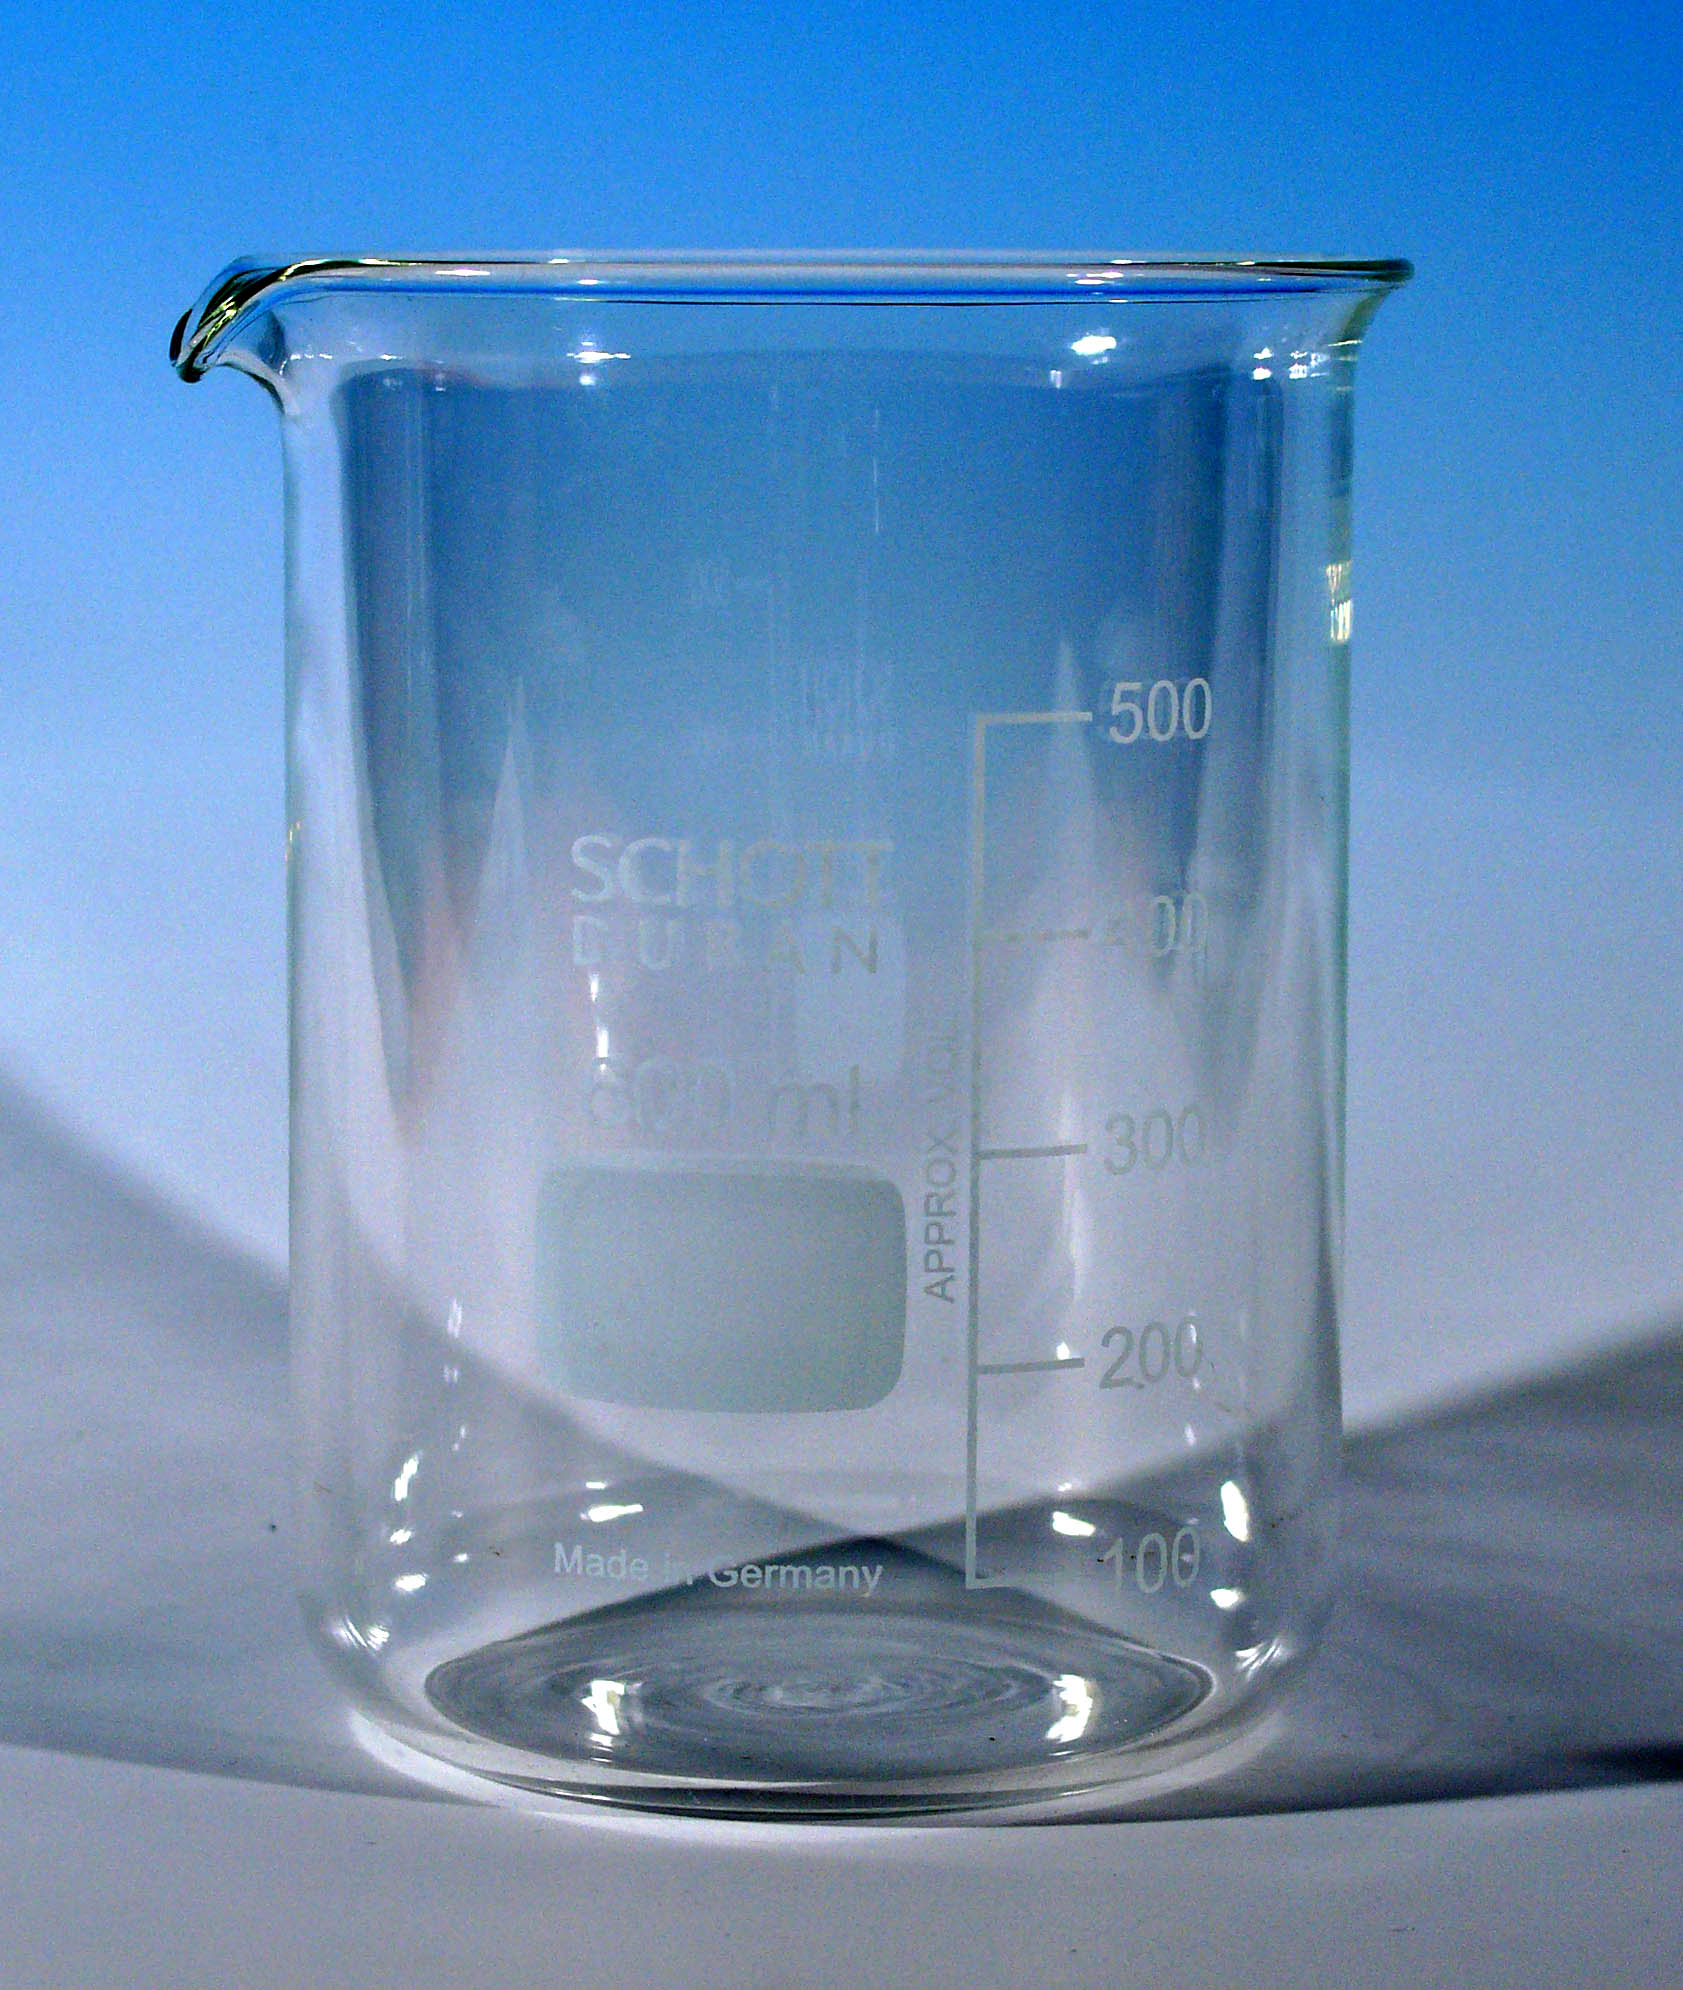
\includegraphics[width=4cm, height=4cm]{chapter1/figure1-15}} node[rotate=90, font=\tiny] at ([yshift=.5cm,xshift=.1cm]a.south east) {\textsuperscript{\textcopyright} wikipedia} ;
\node[text width=5cm] at ([yshift=0.2cm]a.north) {\mytriangle{red}Beakers can carry a liquid volume};
\end{tikzpicture}
\begin{tikzpicture} \node (a) at (0,0) {\includegraphics[width=4cm, height=4cm]{chapter1/figure1-16}} node[rotate=90, font=\tiny] at ([yshift=.5cm,xshift=.1cm]a.south east) {\textsuperscript{\textcopyright} PngImg} ;
\node[text width=5cm] at ([yshift=0.2cm]a.north) {\mytriangle{red}Thermometers measure temperature};
\end{tikzpicture}
\begin{tikzpicture} \node (a) at (0,0) {\includegraphics[width=4cm, height=6cm ]{chapter1/figure1-17}} node[rotate=90, font=\tiny] at ([yshift=.5cm,xshift=.1cm]a.south east) {\textsuperscript{\textcopyright} www.weberscientific.com} ;
\node[text width=5cm] at ([yshift=0.2cm]a.north) {\mytriangle{red}pipets are used in chemistry practice to add an exact volume of liquid};
\end{tikzpicture}
%\caption{Examples of measuring equipment}
\label{fig:marginfig2}
\end{marginfigure}








\begin{example} % EXAMPLE BOX
State the type of measurement indicated in each of the following:
\begin{multicols}{4}
\begin{enumerate}[label=(\alph*)]
\item 1foot
\item 20Kg
\item 3L
\item 300K
\end{enumerate}
\end{multicols}
\textlcsc{ \textcolor{dgreen}{\Large \textbf{Solution}} }\\
(a) length; (b) mass; (c) volume; (d) temperature; 
\\
\faDiamond\ \textlcsc{ \textcolor{dgreen}{\Large \textbf{Study Check}} }\\
State the type of measurement indicated in each of the following:
\begin{multicols}{4}
\begin{enumerate}[label=(\alph*)]
\item 800F
\item 1$\text{m}^3$
\item 3m
\item 67s
\end{enumerate}
\end{multicols}
\flushright Answer: (a) temperature; (b) volume; (c) length; (d) time;
\end{example}% EXAMPLE BOX ALTERNATIVE




\refstepcounter{table} \label{tab:units1}
%\begin{table}[ht]
\fontfamily{ppl}\selectfont
\begin{tabular}{llll}
\rowcolor{black!45}
\toprule
\multicolumn{4}{l}{\hypersetup{colorlinks,linkcolor={white}} \cellcolor{black}\color{white}\bfseries\small Table \ref{tab:units1} Different unit systems } \\
\midrule
Measuremts & Metric System & International System (SI)& English System \\
\midrule
Length & Meter (m) & Meter (m)& Foot (f)\\
 Volume & Liter (L)  &  Cubic meter ($\text{m}^3$)& Gallon (gal) \\
   Mass & Gram (g)  &  Kilogram (kg)& Pound (lb)\\
  Time&  Second (s) & Second (s) &Second (s)  \\
 Temperature &Celsius ($^{\circ}$C)   & Kelvin (K)& Fahrenheit ($^{\circ}$F)  \\
\bottomrule
\end{tabular}
%\end{table}

\section{Prefixes \& Conversion Factors}


Let\textquotesingle s consider the following measurements: 1 \begin{bf}k\end{bf}m, 2 \begin{bf}c\end{bf}m, and 3 m that can be read as one kilometer, two centimeters, and three meters. The word kilo (\begin{bf}k\end{bf}) and centi (\begin{bf}c\end{bf}) are called prefixed whereas meter (m) is a simple unit. Kilometer is larger than meter, whereas centimeter is smaller than a meter. Prefixes such as kilo or centi are attached to units in order to make numbers more manageable. For example, the radius of the earth is 6356 km, and this number is easier to handle than 6356000m. At the same time, we can attach any prefix to different units. Hence, we can talk about a centimeter (\begin{bf}c\end{bf}m) but also about a centisecond (\begin{bf}c\end{bf}s) or centiliter (\begin{bf}c\end{bf}L). All these units have the same prefix. Table \ref{tab:units1} lists some of the metric prefixes, their symbols, and their decimal values.





\begin{center}
\refstepcounter{table} \label{tab:units2}
%\begin{table}[ht]
\fontfamily{ppl}\selectfont
\begin{tabular}{lllll}
\rowcolor{black!45}
\toprule
\multicolumn{5}{l}{\hypersetup{colorlinks,linkcolor={white}} \cellcolor{black}\color{white}\bfseries\small Table \ref{tab:units2} Different prefixes } \\
\midrule
Prefix & Symbol&\multicolumn{2}{c}{Meaning} & Value \\
\midrule
peta & \multicolumn{1}{c}{P}  &\multicolumn{1}{r}{1000000000000000}&   &$1\times10^{15}$  \\
tera & \multicolumn{1}{c}{T}  &\multicolumn{1}{r}{1000000000000}&   &$1\times10^{12}$  \\
giga & \multicolumn{1}{c}{G}  &\multicolumn{1}{r}{1000000000}&&$1\times10^9$  \\
mega & \multicolumn{1}{c}{M}  &\multicolumn{1}{r}{1000000}&&$1\times10^6$  \\
kilo & \multicolumn{1}{c}{k}  &\multicolumn{1}{r}{1000}&&$1\times10^3$  \\
hecto & \multicolumn{1}{c}{h}  &\multicolumn{1}{r}{100}&&$1\times10^2$  \\
deca & \multicolumn{1}{c}{da}  &\multicolumn{1}{r}{10}&&$1\times10^1$  \\
\midrule
--&  \multicolumn{1}{c}{--}  &&\multicolumn{1}{l}{1}&$1\times10^{0}$  \\
\midrule
deci & \multicolumn{1}{c}{d}  &&\multicolumn{1}{l}{0.1}&$1\times10^{-1}$  \\
centi & \multicolumn{1}{c}{c}  &&\multicolumn{1}{l}{0.01}&$1\times10^{-2}$  \\
milli & \multicolumn{1}{c}{m}  &&\multicolumn{1}{l}{0.001}&$1\times10^{-3}$  \\
micro & \multicolumn{1}{c}{$\mu$}  &&\multicolumn{1}{l}{0.00001}&$1\times10^{-6}$  \\
nano & \multicolumn{1}{c}{n}  &&\multicolumn{1}{l}{0.000000001}&$1\times10^{-9}$  \\
pico & \multicolumn{1}{c}{p}  &&\multicolumn{1}{l}{0.000000000001}&$1\times10^{-12}$  \\
femto & \multicolumn{1}{c}{f } &&\multicolumn{1}{l}{0.000000000000001}&$1\times10^{-15}$  \\
\bottomrule
\end{tabular}\end{center}
%\caption{Table containing some Prefixes. For example, 1km is a thousand ($1\times 10^{3}$) meters, and 1ms is ($1\times 10^{-3}$) seconds. The prefixes on top of the table are larger than the unit, and for examples 1Tbyte is larger than a byte. The prefixed on the bottom are smaller than the unit, and 1fs is smaller than a second.}
%\label{table1:2}
%\end{table}
%\resizeableyellownote{2.5}{1}{Add Table \ref{table1:2} to your flashcard.}




 



\sloppy
\begin{description}
\item[\docfilehook{How to identify prefixes?}{How to identify prefixes?}] Look for example at the measurement 2 cm. Centi (c) is the prefix and means $1\times10^{-2}$ and meter (m) is the unit which refers to length. Another example, 7 kg means kilogram. Kilo (k) is the prefix and means $1\times10^{3}$, whereas gram (g) is the unit that refers to mass. The prefix refers to the first letter whereas the unit refers to the last letter. \\
Would you prefer to be paid a kilodollar, a dollar or a centidollar? A unit with a prefix can be bigger or smaller than the plain unit--this is the unit without prefix--, depending on the prefix. The following prefixes make the unit smaller: deci, centi, milli, micro, nano, pico and femto. For example a fs (femtosecond) is smaller than a s (second). Differently, the following prefixes make the unit larger: Tera, Giga, Mega. For example a Tb (terabyte) is larger than a b (byte). byte is a unit used in computer science.
\marginnote{\faBicycle\ Remember: the \textcolor{blue}{ \textbf{pre}}fix always comes first as the \textcolor{blue}{ \textbf{c}} in \textcolor{blue}{ \textbf{c}}m}
%\begin{figure*}[h] % FUL FIGURE
%\begin{tikzpicture} \node (a) at (0,0) {\includegraphics[width=\linewidth,scale=0.5]{./chapter1/figure1-4}} node[rotate=90, font=\tiny] at ([yshift=.5cm,xshift=.1cm]a.south east) {\textsuperscript{\textcopyright} wikipedia} ;\end{tikzpicture}
%\caption{The different scales of the matter}
%\end{figure*}

\item[\docfilehook{How to write unit equalities and conversion factors}{How to write unit equalities and conversion factors}] Unit equalities are simple expressions that relate a unit with a unit with prefix. For example: one centimeter (cm) is $1\times10^{-2}$m. Hence we can write this as a unit equality:
\begin{equation*}
\boxed{   1cm=1\times10^{-2}m}\text{ unit equality}    
\end{equation*}
Let\textquotesingle s compare cm and m. The first, cm, is a unit with a prefix, whereas m is simple a unit of length without a prefix. In order know how many m are there in a cm we need to write down a conversion factor. Think about prefixes as synonymous of a number. In this way, centi stands for  $1\times10^{-2}$, so
\marginnote{\faBicycle\ Remember: \textcolor{blue}{ \textbf{equalities}}  are written in line whereas \textcolor{blue}{ \textbf{conversion factors}}  with a fraction.}


\begin{equation*}
\boxed{   \frac{1cm}{1\times10^{-2}m}\ \enspace \text{ or  } \enspace \frac{1\times10^{-2}m}{1cm} }  \  \text{ conversion factor}   
\end{equation*}
 \end{description}
%\resizeableyellownote{2.5}{1}{Add Table \ref{table1:3} to your flashcard.}








%   \begin{marginfigure}
%\begin{tikzpicture} \node (a) at (0,0) {\includegraphics[width=4cm]{chapter1/figure1-5}} node[rotate=90, font=\tiny] at ([yshift=.5cm,xshift=.1cm]a.south east) {\textsuperscript{\textcopyright} wikipedia} ;
%\end{tikzpicture}
%\caption{How many mL do you add to your eye?}
%\label{fig:marginfig5}
%\end{marginfigure}



\begin{example} % EXAMPLE BOX
Complete each of the following equalities and conversion factors:

\begin{multicols}{2}
\begin{enumerate}[label=(\alph*)]
\item 1dm=$\hlmath{\hspace{35pt }}$m
\item 1km=$\hlmath{\hspace{35pt }}$m
\item  $\dfrac{1nm}{\hlmath{\hspace{35pt }}m}$
\item  $\dfrac{\hlmath{\hspace{35pt }}m}{1cm}$

\end{enumerate}
\end{multicols}
\textlcsc{ \textcolor{dgreen}{\Large \textbf{Solution}} }\\
(a) 1dm=$1\times10^{-1}m$; (b) 1km=$1\times10^{3}m$; (c) $\dfrac{1nm}{1\times10^{-9}m}$; (d) $\dfrac{1\times10^{-2}m}{1cm}$; 
\\
\faDiamond\ \textlcsc{ \textcolor{dgreen}{\Large \textbf{Study Check}} }\\
Second is a unit of time. Complete each of the following equalities and conversion factors involving seconds:
\begin{multicols}{3}
\begin{enumerate}[label=(\alph*)]
\item 1cs=$\hlmath{\hspace{35pt }}$s
\item $\dfrac{\hlmath{\hspace{35pt }}s}{1Ts}$
\item $\dfrac{\hlmath{\hspace{35pt }}s}{1Ms}$
\end{enumerate}
\end{multicols}
\flushright Answer: (a) 1cs=$1\times10^{-2}s$; (b) $\dfrac{ 1\times10^{12} s}{1Ts}$; (c) $\dfrac{ 1\times10^{6} s}{1Ms}$;
\end{example}% EXAMPLE BOX ALTERNATIVE




\section{Using Conversion Factors}


Unit equalities in the form of conversion factors are used to convert a unit into another. Sometimes one wants to get rid of a prefix, such as when we transform centimeter (cm) into meter (m). Sometimes, one wants to convert a prefix into another prefix. An example would be converting centimeters (cm) to millimeters (mm). Let\textquotesingle s work on some example.

\begin{description}
\item[\docfilehook{Removing or adding prefixes}{Removing or adding prefixes}] Imagine that you need to remove a prefix from a unit, and convert 3 km (we will call this one the original unit) in meters (this is the final unit). First, you would need the conversion factor corresponding to the prefix (centi) from Table \ref{tab:units2}. Then you need to arrange the conversion factor placing the prefix at the bottom of the fraction. This will cancel out the prefix in the original unit and in the bottom part of the conversion factor, hence leaving the final unit on top of the conversion factor. The arrangement would be:
\begin{equation*}
3\cancel{km} \times \dfrac{1\times10^{3}m}{1\cancel{km}}=3000m
\end{equation*}
Imagine now that you need to add a prefix into a unit, and convert 4000 m in km. The same would apply for this case, but now you will have to arrange the conversion factor so that the prefix is on the top:
\begin{equation*}
4000\cancel{m} \times \dfrac{\text{1 km}}{1\times10^{3}\cancel{m}}=4km
\end{equation*}


%
%   \begin{marginfigure}
%\begin{tikzpicture} \node (a) at (0,0) {\includegraphics[width=4cm]{chapter1/figure1-6}} node[rotate=90, font=\tiny] at ([yshift=.5cm,xshift=.1cm]a.south east) {\textsuperscript{\textcopyright} wikipedia} ;
%\end{tikzpicture}
%\caption{Rulers normally have the cm and inch conversion written.}
%\label{fig:marginfig6}
%\end{marginfigure}


\begin{example} % EXAMPLE BOX
The length of a textbook page is 20cm. Convert 20cm to m.\\
\textlcsc{ \textcolor{dgreen}{\Large \textbf{Solution}} }\\
In order to convert 20cm into meters, we need to remove the prefix (centi) leaving the unit (meter) without any prefix. We will use the conversion factor that relates m to cm:$\dfrac{1\times10^{-2}m}{1cm}$ or $\dfrac{1cm}{1\times10^{-2}m}$. We will arrange the conversion factor so that cm cancels giving m and hence we will use $\dfrac{1\times10^{-2}m}{1cm}$:
 \begin{equation*}
20\cancel{cm} \times \dfrac{1\times10^{-2}m}{1\cancel{cm}}=0.2m
\end{equation*}
The original units and on the bottom of the conversion factor cancel and we get meters, the final unit.
\\
\faDiamond\ \textlcsc{ \textcolor{dgreen}{\Large \textbf{Study Check}} }\\
Convert 100m to km.
\flushright Answer:$100\cancel{m} \times \dfrac{km}{1\times10^{3}\cancel{m}}=0.1km$.
\end{example}% EXAMPLE BOX ALTERNATIVE


\item[\docfilehook{Switching prefixes}{Switching prefixes}] In order to switch a prefix into another prefix, such as transforming 30 millimeters (30 mm) into centimeters (cm), you will need two different conversion factors: the first conversion factor will remove the original unit (mm) introducing an intermediate unit, meters (m), whereas the second conversion factor will remove the intermediate meter and introduce the final unit (cm). You will get the conversion factors from Table \ref{tab:units2}. You will arrange the first conversion factor so that the original unit cancels out with the bottom of the first conversion factor, giving you an intermediate unit. You will arrange the second conversion factor so that the intermediate unit cancels out with the bottom of the second conversion factor giving the final unit. For this example:
 \begin{equation*}
30\cancel{mm} \times \dfrac{1\times10^{-3}\cancel{m}}{1\cancel{mm}}   \times \dfrac{1cm}{1\times10^{-2}\cancel{m}}       =3cm
\end{equation*}

\marginnote{\faBicycle\ Remember: the number $1\times 10^{-3}$ is \textcolor{blue}{ \textbf{scientific notation}} and must be typed in the calculator as: 1\keystroke{EE}$-3$.}
\begin{example} % EXAMPLE BOX
The length of a textbook page is 20cm. How many mm correspond this length.\\
\textlcsc{ \textcolor{dgreen}{\Large \textbf{Solution}} }\\
 We want to convert 20 cm into mm, that is, we are switching prefixed. In order to do this, you need two conversion factors:$\dfrac{1\times10^{-2}m}{1cm}$ and $\dfrac{1\times10^{-3}m}{1mm}$. You will have to arrange the number (20cm) and the two conversion factors in the following form:
 \begin{equation*}
20\cancel{cm} \times \dfrac{1\times10^{-2}\cancel{m}}{1\cancel{cm}}   \times \dfrac{1mm}{1\times10^{-3}\cancel{m}}       =200mm
\end{equation*}

\faDiamond\ \textlcsc{ \textcolor{dgreen}{\Large \textbf{Study Check}} }\\
Convert 100mm to km.
\flushright Answer:$100\cancel{mm} \times \dfrac{1\times10^{-3}\cancel{m}}{1\cancel{mm}}   \times \dfrac{1km}{1\times10^{3}\cancel{m}}       =1\times 10^{-4}km$.
\end{example}% EXAMPLE BOX ALTERNATIVE



   

   
   





\marginnote{\faBicycle\ Remember: if you use a power on a power of ten, the power and the ten exponent multiplies, and for example $1\times (10^{-2})^2$ is $1\times 10^{-4}$ or $1\times (10^{-4})^3$ is $1\times 10^{-12}$. Also the power key in your calculator is \keystroke{\Large \^} }
\item[\docfilehook{Square or cubic units}{Square or cubic units}] How big is your apartment? You might be living in a 750$ft^2$ loft in Brooklyn or in a larger house Upstate. Often times we encounter cubic or square units such as cubic centimeter ($cm^3$) or square feet ($ft^2$). The equivalencies for cubic or square units should take into account the unit power (power of two or power of three). 
If $1cm=1\times 10^{-2}m$, for square units the relation should be squared and $1cm^2=1\times (10^{-2})^2m^2=1\times 10^{-4}m^2$. Another example, for the case of mm and $mm^3$:
\begin{equation*}
\boxed{   \frac{1mm}{1\times10^{-3}m}\ \enspace \text{ and  } \enspace \frac{1mm^3}{1\times10^{-9}m^3}}     
\end{equation*}
Let us work on an example in which we want to convert $30m^2$ into $m^2$:
 \begin{equation*}
30\cancel{\text{m}^2} \times \dfrac{1cm^2 }{1\times10^{-4}\cancel{m^2}}=3\times 10^{5}cm^2
\end{equation*}

\begin{example} % EXAMPLE BOX
How many $m^2$ is 20$cm^2$.\\
\textlcsc{ \textcolor{dgreen}{\Large \textbf{Solution}} }\\
In order to convert 20$cm^2$ to square meters, we need to remove the centi prefix and that will give us the unit square meter without any prefix. We will use the conversion factor that relates $m^2$ to $cm^2$:$\dfrac{1\times10^{-4}m^2}{1cm^2}$ or $\dfrac{1cm^2}{1\times10^{-4}m^2}$. 
 \begin{equation*}
20\cancel{cm^2} \times \dfrac{1\times10^{-4}m^2}{1\cancel{cm^2}}=2\times 10^{-3}m^2
\end{equation*}
\faDiamond\ \textlcsc{ \textcolor{dgreen}{\Large \textbf{Study Check}} }\\
Convert 100$m^3$ to $dm^3$.
\flushright Answer:$100\cancel{m^3} \times \dfrac{1dm^3}{1\times10^{-3}\cancel{m^3}}=1\times 10^5dm^3$.
\end{example}% EXAMPLE BOX ALTERNATIVE



%\begin{marginfigure}
%\begin{tikzpicture} \node (a) at (0,0) {\includegraphics[width=4cm, height=4cm]{chapter1/figure1-7}} node[rotate=90, font=\tiny] at ([yshift=.5cm,xshift=.1cm]a.south east) {\textsuperscript{\textcopyright} wikipedia} ;
%\node[text width=5cm] at ([yshift=0.2cm]a.north) {\mytriangle{red}The per-feet-square price in Tribeca where The Borough of Manhattan Community College is located in NYC is $\$1,750$};
%\end{tikzpicture}
%\begin{tikzpicture} \node (a) at (0,0) {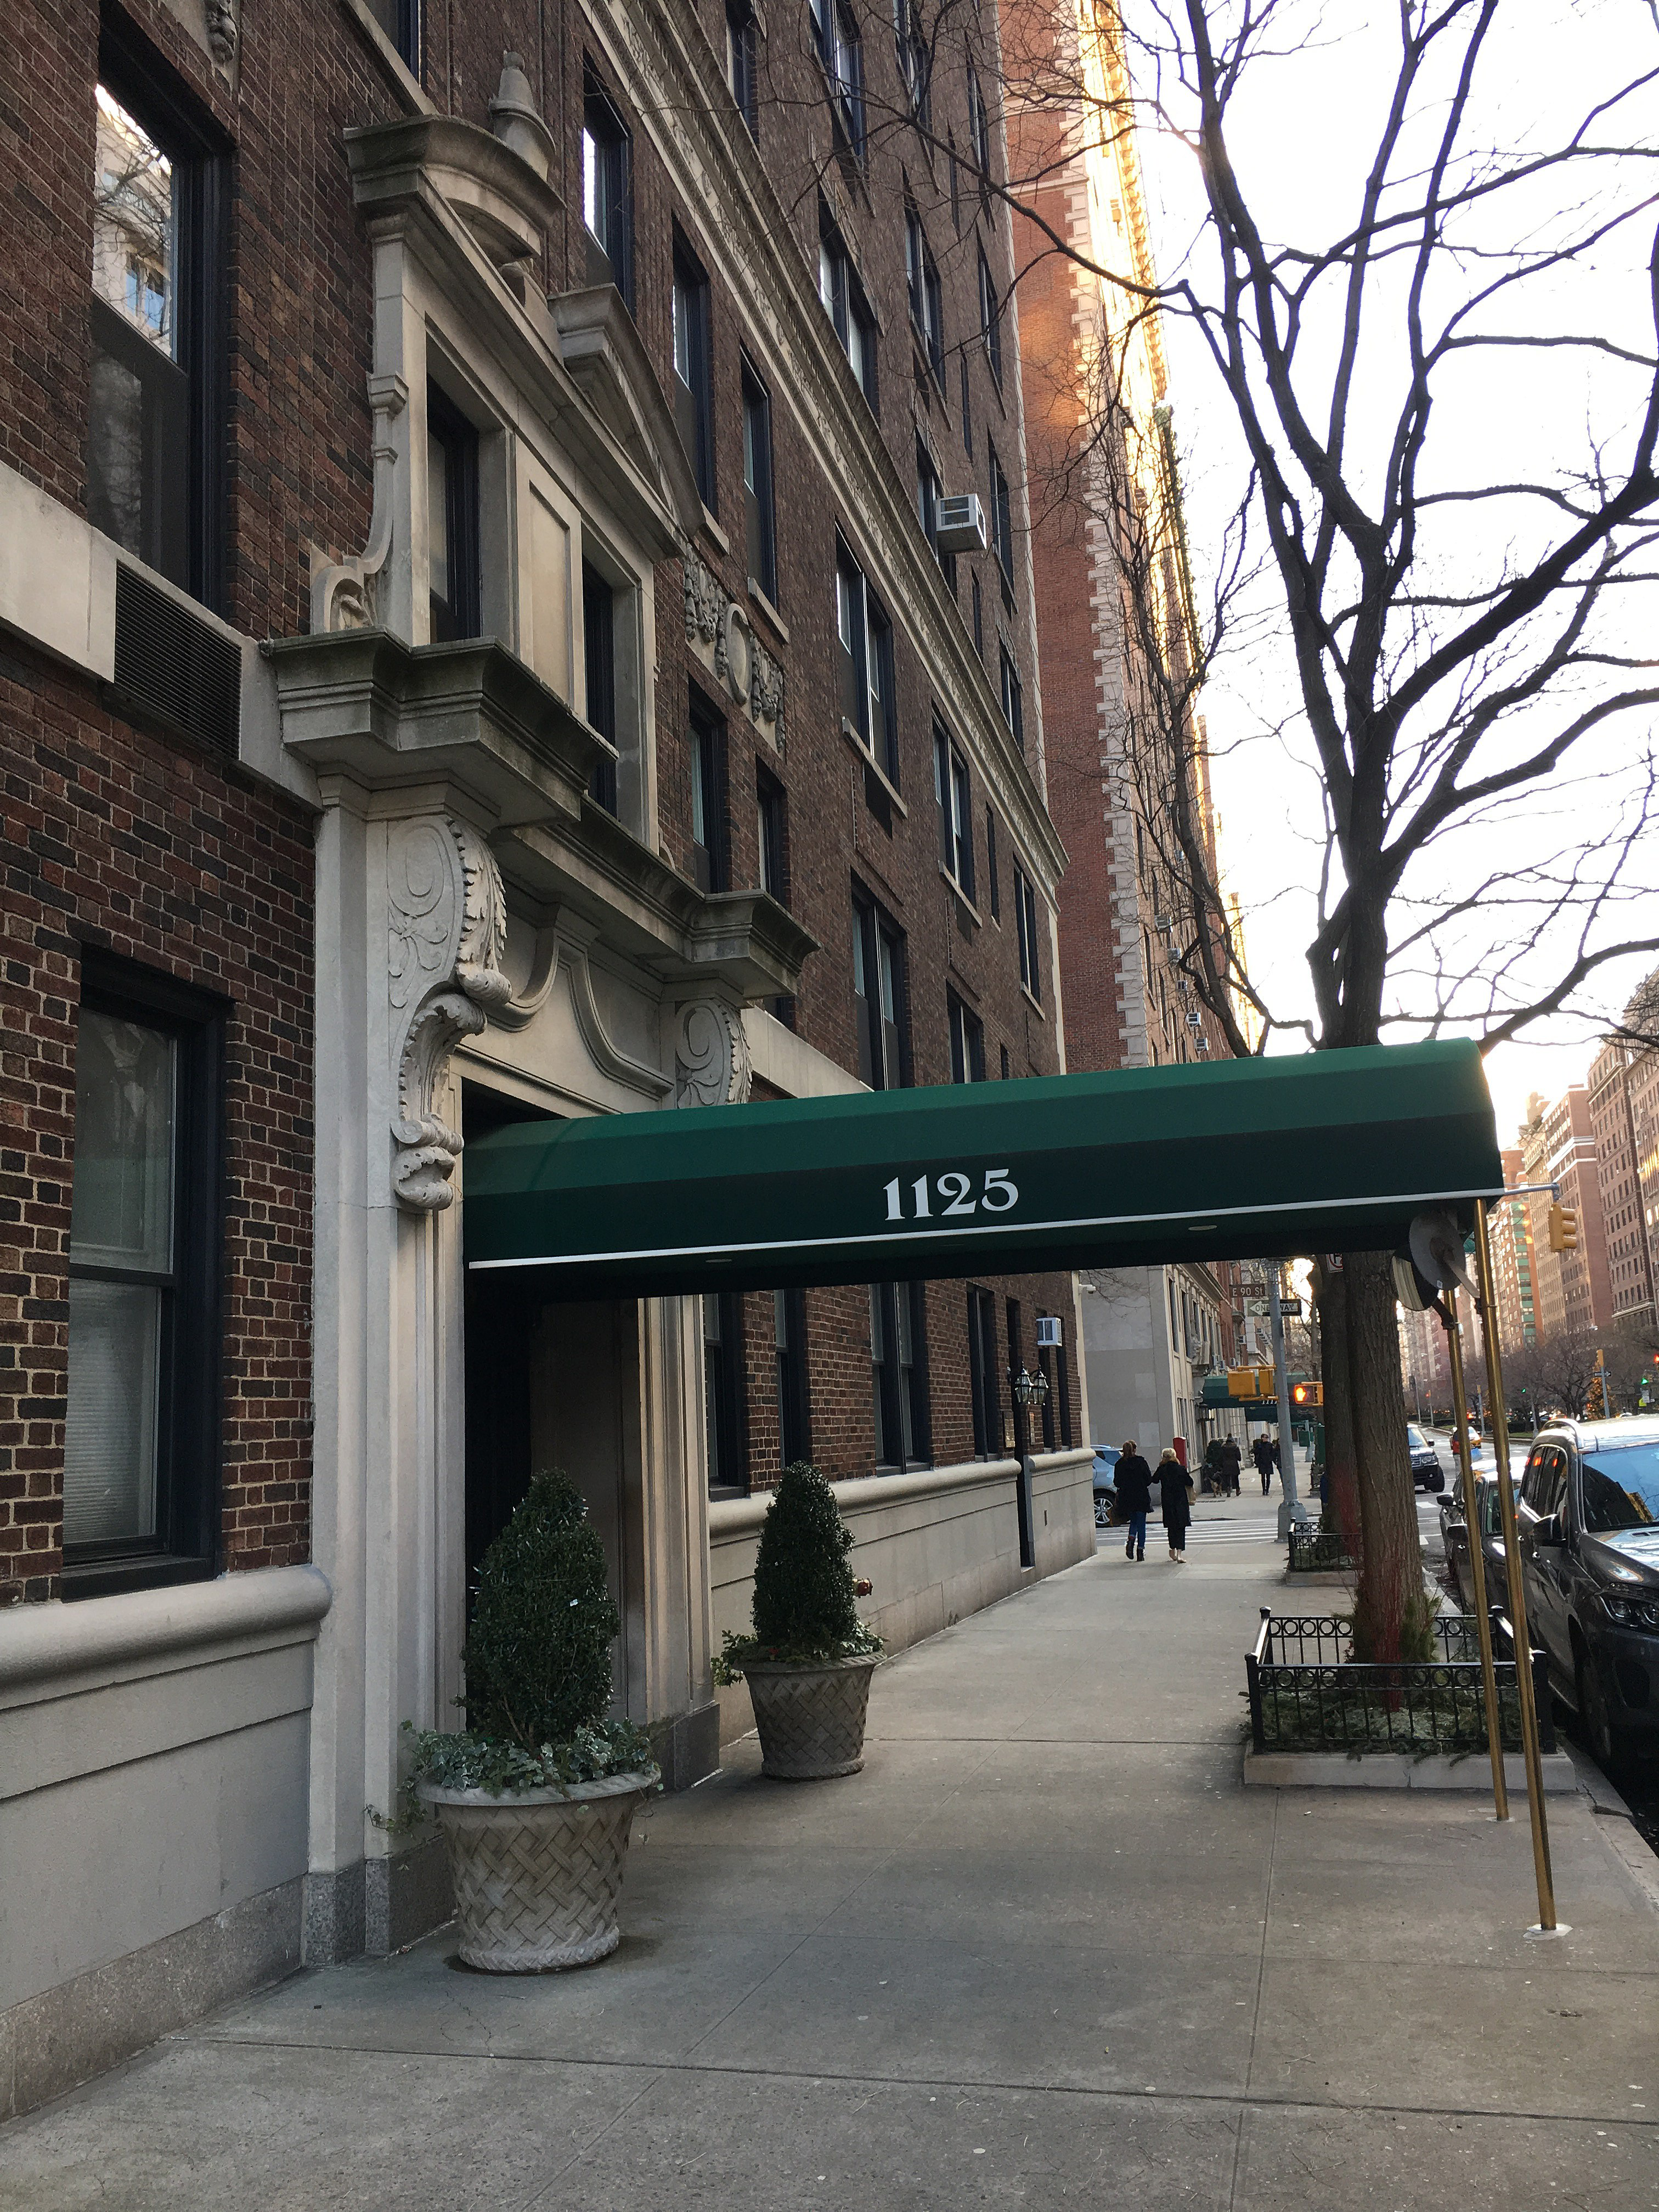
\includegraphics[width=4cm, height=4cm]{chapter1/figure1-18}} node[rotate=90, font=\tiny] at ([yshift=.5cm,xshift=.1cm]a.south east) {\textsuperscript{\textcopyright} wikipedia} ;
%\node[text width=5cm] at ([yshift=0.2cm]a.north) {\mytriangle{red}The per-feet-square price in the upper east side of NYC is $\$1,408$};
%\end{tikzpicture}
%
%
%\caption{The per-feet-square price in Tribeca where The Borough of Manhattan Community College is located in NYC is $\$1,750$}
%\label{fig:marginfig7}
%\end{marginfigure}










\item[\docfilehook{Units of volume}{Units of volume}] Units such as L or mL are units of volume. As volume is a three-dimensional property, those units somehow have to be related to the units of length. In fact one liter is the same as one $dm^3$ and one ml is the same as one $cm^3$. In the allied health field, the units \emph{mL} is also written as \emph{cc} as in cubic centiliters.
\begin{equation*}
\boxed{   1L=1dm^3 \enspace \text{and}  \enspace1mL=1cm^3}   
\end{equation*}

Let us work on an example in which we want to convert $30cm^3$ into L:
 \begin{equation*}
30\cancel{\text{cm}^3} \times \dfrac{1\cancel{mL} }{1\cancel{cm^3}}\times \dfrac{1\times 10^{-3}L }{1\cancel{mL}} =3\times 10^{-2}L
\end{equation*}


\begin{example} % EXAMPLE BOX
Convert 30 $m^3$ into L.\\
\textlcsc{ \textcolor{dgreen}{\Large \textbf{Solution}} }\\
In order to convert $m^3$ into L we just need to remember that the L actually refers to $dm^3$, therefore is connected to meter. We will first convert $m^3$ into $dm^3$ and then $dm^3$ into L.
 \begin{equation*}
30\cancel{m^3} \times \dfrac{1 \cancel{dm^3}}{1\times10^{-3}\cancel{m^3}}   \times  \dfrac{1L}{1\cancel{dm^3}} =3\times 10^{4}L
\end{equation*}
\faDiamond\ \textlcsc{ \textcolor{dgreen}{\Large \textbf{Study Check}} }\\
Convert 40L to $cm^3$.
\flushright Answer: $40\cancel{L} \times \dfrac{1\cancel{mL}}{1\times10^{-3}\cancel{L}} \times \dfrac{1cm^3}{1\cancel{mL}}=4\times 10^4cm^3$.
\end{example}% EXAMPLE BOX ALTERNATIVE

\item[\docfilehook{Using other equalities}{Using other equalities}] How many hours is 300 minutes, or how many centimeters is 2 inches? Some of the units conversion are not based on a power of ten relationship such as the ones in Table \ref{tab:units2}. Table \ref{tab:units3} lists some of the common equalities that can be easily converted into conversion factor. As an example, the unit equivalency between hours and minutes is $60min=1h$ and the conversion factor would be $\dfrac{60min}{1h}$ or $\dfrac{1h}{60min}$.
\refstepcounter{table} \label{tab:units3}
\begin{center}
\fontfamily{ppl}\selectfont
\begin{tabular}{ll}
\rowcolor{black!45}
\toprule
\multicolumn{2}{l}{\hypersetup{colorlinks,linkcolor={white}} \cellcolor{black}\color{white}\bfseries\small Table \ref{tab:units3} Table containing some common unit equalities } \\
\midrule
Unit & Equality \\
\midrule
Inches (in)-centimeters (cm)  &$2.54\text{ cm}=1\text{ in}$  \\
miles (mi)-meters ($m$)  &$1\text{ mi}=1609.34$m  \\
minutes (min)-hours (h)  &$60\text{ min}=1\text{ h}$  \\
minutes (min)-seconds (s)  &$60\text{ s}=1\text{ min}$  \\
pound (lb)-grams (g)  &$454\text{ g}=1\text{ lb}$  \\
cubic centimeter ($cm^3$)-mililiters (mL)  &$1\text{ mL}=1\text{cm}^3$  \\
Liter (L)-cubic decimeters ($dm^3$)  &$1\text{ L}=1\text{dm}^3$  \\
drops-mililiters (mL)  &$1\text{ mL}=15\text{ drops}$  \\
\bottomrule
\end{tabular}
\end{center}


\begin{example} % EXAMPLE BOX
Convert 20 in to cm.\\
\textlcsc{ \textcolor{dgreen}{\Large \textbf{Solution}} }\\
 We want to convert 20 inches into centimeters. The relationship between Inch and centimeter is given in Table \ref{tab:units3}. In order to do this, you need the conversion factor:$\dfrac{1in}{2.54cm}$ or $\dfrac{2.54cm}{1in}$. You will have to arrange the number (20 in) and the conversion factor in the following form:
 \begin{equation*}
20\cancel{in} \times \dfrac{2.54cm}{1\cancel{in}}=50.80cm
\end{equation*}
\faDiamond\ \textlcsc{ \textcolor{dgreen}{\Large \textbf{Study Check}} }
Convert 200mL to drops.
\flushright Answer: $200\cancel{mL} \times \dfrac{15 drops}{1\cancel{mL}}=3000drops=3\times 10^3drops$
\end{example}% EXAMPLE BOX ALTERNATIVE

\end{description}


\section{Significant Figures}
Exact numbers results from counting. For example, think about how many eggs are there in your refrigerator, there might be three and this number is an exact number.
Differently, numbers that results from a measurement are called measured values and they are subject to uncertainty--in another words error.  For example, if you weight a single egg in an scale depending of the type of scale you used you will measure 70g or 71g or maybe 70.8g. The mass of an egg is a measured property and hence some of the digits of the measurement are uncertain. The goal of this section is, given a value, calculate the number of significant figures of a number (we will refer to significant figures as SF, or SFs). Another goal is to estimate significant figures in calculation in order to express the result with the right number of digits and significant figures.

\begin{description}
\item[\docfilehook{Significant figures of numbers}{Significant figures of numbers}] In general all numbers different than zero are significant and for example the number 123 has three significant figures. Similarly, the number 45 has two significant figures. Zeros are also significant except when:\\
 \faCodeFork\ \begin{bf}Exception 1\end{bf}  \begin{it}A zero is not significant when placed at the beginning of a decimal number. \end{it} \\
 For example, the number 0.123 has three significant figures, as the first zero is not significant. Similarly, the number 0.002340 has four significant figures as the first three zeros are not significant but the last zero it is. Mind the rule affects only the zeros at the beginning. A final example:
 \begin{equation*}
   0.032 \enspace \text{(2SF)}  
\end{equation*}

 \faCodeFork\ \begin{bf}Exception 2\end{bf} \begin{it}A zero is not significant when used as a placeholder in a number without a decimal point. \end{it} \\
 For example, the number 1000 has only one significant figure, and the number 3400 has two. Let us consider more examples. The number 120 has two significant figures, as according to the second rule the last zero is not significant. Differently, the number 1203 has four significant figures, as the zero in between two numbers is not affected by neither the first nor the second rule. A final example,
  \begin{equation*}
   3200 \enspace \text{(2SF)}  
\end{equation*}
\faCodeFork\ \begin{bf}Exception 3\end{bf} \begin{it}A zero in a number expressed on scientific notation is significant \end{it} \\
 For example the zero  in $3.0\times 10^{-2}$ is significant, and the number has 2SFs. A final example:
  \begin{equation*}
   3.2020\times 10^{2} \enspace \text{(5SF)}  
\end{equation*}



\begin{example} % EXAMPLE BOX
Indicate the number of significant figures in the following numbers: 123, 4567, 1200, 340, 0.001, 0.023 and 0.0405.
\\
\textlcsc{ \textcolor{dgreen}{\Large \textbf{Solution}} }\\
123 has three significant figures, whereas 4567 has four SF. 1200 has only 2SF as the last two zeros are not significant, and 340 has only 2SF as the last zero is not significant. $0.001$ has only one significant figure as the first 3 zeros are not significant and $0.023$ has only two SFs. Finally, $0.0405$ has threee SFs as the first two zeros are not significant but the zero between 4 and 5 is indeed significant.\\
\faDiamond\ \textlcsc{ \textcolor{dgreen}{\Large \textbf{Study Check}} }\\
Indicate the number of significant figures (SFs) in the following numbers: 4560, 0.123, 1000 and 0.0030. \\
\flushright Answer: 4560 has 3SF, 0.123 has 3SF, 1000 has 1SF and 0.0030 has 2SF.
\end{example}% EXAMPLE BOX ALTERNATIVE

\item[\docfilehook{Significant figures in calculations}{Significant figures in calculations}] There are two different rules that allow you to express the result of a calculations with the correct number of figures.

 \faCodeFork\ \begin{bf}Rule 1 ($+\text{ }-$)\end{bf}  \begin{it} For additions or subtractions, the results has the same number of decimal places as the number with the least decimal places in the calculation.\end{it} For example:
\[34.3451+34.5=68.8 \text{ }(+\text{ }- \text{less decimals})\]
If you add $34.3451+34.5$ you will obtain $68.8451$, however, as $34.3451$ has four decimal places (4DP) and $34.5$ has one decimal place (1DP), the result of adding both numbers will have to have only one decimal place, therefore $68.8451$ needs to be rounded to $68.8$ (1DP). Overall, we have:
\[34.3451\text{ (4DP) }+34.5\text{ (1DP) }=68.8 \text{ (1DP) }\]

 \faCodeFork\ \begin{bf}Rule 2 ($\times\text{ }\div$)\end{bf}  \begin{it} For multiplications and divisions, the number of significant figures of the result should be the same as the least number of significant figures involved\end{it}. For example, if you carry the following multiplication:

\[4500 \times 342 =1500000\text{ }(\times\text{ }\div \text{less SFs})\]

the number $4500$ (2SF) has two significant figures, whereas the number $342$ (3SF) has three significant figures. If we multiply both numbers the results should contain just two significant figures. The result of multiplying $4500 \times 342$ is $1539000$ (4SF), however, this number needs to be rounded into two significant figures into 1500000 (2SF). Overall we have:

\[4500 \text{ (2SF) } \times 342\text{ (3SF) } =1500000 \text{ (2SF) }\]


\begin{example} % EXAMPLE BOX
Do the following calculation with the correct number of figures.
\begin{equation*}
\dfrac{88.5-87.57}{345.13\times100}
\end{equation*}
\textlcsc{ \textcolor{dgreen}{\Large \textbf{Solution}} }\\
We will analyze each number indicating the number of SF and Digits (DP): 88.5(3SF, 1DP), 87.57(4SF, 2DP),  345.13(6SF, 2DP) and  100(1SF, 0DP). The result of doing the addition needs to be rounded to one single decimal place: $88.5-87.57=0.93\simeq 0.9$. After that we have only multiplications and divisions and hence we will now focus on the number of SFs:
\begin{equation*}
\dfrac{0.9\text{ (1SF) }}{345.13\text{ (5SF) }\times100\text{ (1SF) }}
\end{equation*}
The result of this operation needs to be rounded to one SF:
\begin{equation*}
\dfrac{0.9}{345.13\times100}=2.6077\times 10^{-5} \simeq 3\times 10^5\text{ (1SF) }
\end{equation*}
\faDiamond\ \textlcsc{ \textcolor{dgreen}{\Large \textbf{Study Check}} }\\
Do the following calculation with the correct number of figures: $(24.56+2.433)\times0.013$
\flushright Answer: 0.35
\end{example}% EXAMPLE BOX ALTERNATIVE





\end{description}
\newpage
\section{Matter and density}

We can classify chemical substances in terms of what they are made of. Some are made of just one thing, others contain different components. At the same time, some substances look like they are made of one thing and indeed they are made of many components. This section covers the classification of matter according to the purity of substances and mixtures. It also elaborates on the types of mixtures one can find. The final part of the section deals with density.
\stepcounter{figurenewcounter}   \refstepcounter{figure}  \label{Fig:{\chapterlabel}\thefigurenewcounter}
%\caption{Classification of the matter}
\hspace{-5cm}\vspace{-0.5cm}
\begin{minipage}[b]{1.\linewidth}
\begin{center}
\resizebox{1.3\textwidth}{!}{
\begin{tikzpicture}
  [
    start chain=p going below,
    every on chain/.append style={etape},
    every join/.append style={line},
    node distance=1 and .85,
  ]
  {
    \node (a) [on chain, join] {All Matter}; \node[text width=4cm, , font=\small] at ([yshift=-.7cm]a.south){Variable composition?};
    
    
    {[start branch=r going below right] \node (b) [on chain] {Pure Substance};\node[text width=4cm, font=\small] at ([yshift=-.7cm, xshift=.4cm]b.south){Different types of atoms?};}
    {[continue branch=r going below right] \node (b1) [on chain,xshift=-2cm] {Compounds};\node[font=\small] at ([yshift=.5cm, xshift=.4cm]b1.north){Yes};}{[continue branch=r going left] \node (b2) [on chain,xshift=-0cm] {Elements};\node[font=\small] at ([yshift=.5cm, xshift=-.4cm]b2.north){No};}%\node [on chain, join] {Atoms};
    {[start branch=l going below left] \node (c) [on chain] {Mixture};\node[text width=4cm,  font=\small] at ([yshift=-.7cm, xshift=.4cm]c.south){Distinguishable parts?}; }
    {[continue branch=l going below right] \node (c1) [on chain,xshift=-2cm] {Heterogeneous};\node[font=\small] at ([yshift=.5cm, xshift=.4cm]c1.north){Yes};}{[continue branch=l going left] \node (c2) [on chain,xshift=-0cm] {Homogeneous};\node[font=\small] at ([yshift=.5cm, xshift=-.4cm]c2.north){No};}
\path [line] (a.south) -- ([yshift=-.5cm]a.south) --  ([yshift=.5cm]b.north) --  (b.north); 
\path [line]  ([yshift=-.5cm]a.south) --  ([yshift=.5cm]c.north) --  (c.north); 
\path [line] (b.south) -- ([yshift=-.5cm]b.south) --  ([yshift=.5cm]b1.north) --  (b1.north); 
\path [line] (b.south) -- ([yshift=-.5cm]b.south) --  ([yshift=.5cm]b2.north) --  (b2.north); 
\path [line] (c.south) -- ([yshift=-.5cm]c.south) --  ([yshift=.5cm]c1.north) --  (c1.north); 
\path [line] (c.south) -- ([yshift=-.5cm]c.south) --  ([yshift=.5cm]c2.north) --  (c2.north); 


 \node (d) at ([yshift=-1.5cm]c1.south) {\includegraphics[width=3cm]{chapter1/figure1-14}} node[rotate=90, font=\tiny] at ([yshift=.5cm,xshift=.1cm]d.south east) {\textsuperscript{\textcopyright} Flirk} ; \node[text width=3cm,font=\small] at ([yshift=-.5cm, xshift=.4cm]d.south){A bowl of fruit loops is an heterogeneous mixture};

 \node (e) at ([yshift=-1.5cm]c2.south) {\includegraphics[width=3cm]{chapter1/figure1-12}} node[rotate=90, font=\tiny] at ([yshift=.5cm,xshift=.1cm]e.south east) {\textsuperscript{\textcopyright} Wallpaperflare} ; \node[text width=3cm,font=\small] at ([yshift=-.5cm, xshift=.4cm]e.south){Brass is a homogeneous mixture of two metals};
  \node (f) at ([yshift=-1.5cm]b1.south) {\includegraphics[width=3cm, height=3cm]{chapter1/figure1-11}} node[rotate=90, font=\tiny] at ([yshift=.5cm,xshift=.1cm]f.south east) {\textsuperscript{\textcopyright} Flickr} ; \node[text width=3cm,font=\small] at ([yshift=-.5cm, xshift=.4cm]f.south){Gold is an element};
 
  \node (g) at ([yshift=-1.5cm]b2.south) {\includegraphics[width=3cm, height=2.5cm]{chapter1/figure1-13}} node[rotate=90, font=\tiny] at ([yshift=.5cm,xshift=.1cm]g.south east) {\textsuperscript{\textcopyright} Pxlfuel} ; \node[text width=3cm,font=\small] at ([yshift=-.5cm, xshift=.4cm]g.south){Water is a compounds made of hydrogen and oxygen};

  }
\end{tikzpicture}
}
\begin{tikzpicture}
 \node[text width=12cm, fontscale=.3,shift={(-0em,2em)}] at (0em,-0em) { \begin{bf}\color{black}\bfseries\large Figure \ref{Fig:{\chapterlabel}\thefigurenewcounter} \end{bf} Classification of the matter };
\end{tikzpicture}
\end{center}\end{minipage}



\begin{description}
\item[\docfilehook{Pure Substances and mixtures}{Pure Substances and mixtures}] \emph{Pure substances} have a definite composition, that is, are only made of one thing. There are two different types of pure substances: elements and compounds. \emph{Elements} are composed of only one type of atom. Examples are silver, iron, and aluminum that all contain one type of substance, and iron is only made of iron atoms, for example. \emph{Compounds} are combinations of different elements. For example, water, \ce{H2O} is made of a combination of hydrogen and oxygen atoms. \emph{Mixtures} are physical combinations of different substances. For example, air is a mixture of oxygen and nitrogen. 
\item[\docfilehook{Types of Mixture}{Types of Mixture}]Mixtures can be homogeneous or heterogeneous. In a \emph{homogeneous mixture}--also known as solutions--the composition is uniform throughout the sample. An example of an homogeneous mixture is air, which contains oxygen and nitrogen or salty water, a solution of salt and water. \emph{Heterogeneous mixtures} are mixtures in which the components are not uniformly distributed throughout the sample. An example would be a chocolate chip cookie in which you can differentiate the dough and the chocolate.




\begin{example} %%%%%%%%%%%%%%%%%%%%%%%% EXAMPLE BOX
Classify as  element, compound, homogeneous mixture, heterogeneous mixture:
\begin{multicols}{4}
\begin{enumerate}[label=(\alph*)]
\item An iron nail
\item Milk
\item Sugar
\item miso soup 
\end{enumerate}
\end{multicols}
\textlcsc{ \textcolor{dgreen}{\Large \textbf{Solution}} }\\
(a) An iron nail is an element as it is only made of iron, a single material; (b) Milk is a homogeneous mixture as it is made of water, fat, protein even though you only see a single substance; (c) Sugar is a compound made of carbon and other constituents; (d) miso soup is a mixture of water, fat and other chemicals and therefore is a mixture. As you can differentiate its constituents we call this heterogeneous mixture.\\
\faDiamond\ \textlcsc{ \textcolor{dgreen}{\Large \textbf{Study Check}} }\\
Classify as  element, compound, homogeneous mixture, heterogeneous mixture:
\begin{multicols}{4}
\begin{enumerate}[label=(\alph*)]
\item muscle milk
\item water
\item a gold ring
\item rice \& beans
\end{enumerate}
\end{multicols}
\flushright Answer: (a) homog. mix.; (b) compound; (c) element; (d) heterog. mix.
\end{example}%%%%%%%%%%%%%%%%%%%%%%%% EXAMPLE BOX



\item[\docfilehook{Density }{Density }] Density refers to the mass of a substance with respect to its volume. This is an unique property for each substance. For example, the density for copper is 8.92 $g\cdot ml^{-1}$ and for gold is 19.3 $g\cdot ml^{-1}$. By measuring density only you would be able to differentiate copper than gold. The larger density the more compact is an object and that means the more mass per volume it has. The formula for density is
%\resizeableyellownote{2.5}{1}{Add  Formula \ref{formula1:1} to your flashcard.}
\begin{equation}
\boxed{   \text{Density}=\frac{\text{Mass of substance}}{\text{Volume of substance}}   }
\label{formula1:1}
\end{equation}

\item[\docfilehook{Density and mixing}{Density and mixing}] A small piece of ice will float on water. The reason for that is density: density of ice (0.9g/mL) is smaller than density of water (1.0g/mL) and hence ice will stay on top of water. Objects with density larger than 1 g/mL will sink whereas objects with density smaller than this value will float. If you add a drop of vegetable oil to a glass of water, the drop will float. This is because the density of oil is smaller than 1g/mL.

\refstepcounter{table} \label{tab:units4}
\begin{center}
\fontfamily{ppl}\selectfont
\begin{tabular}{lll}
\rowcolor{black!45}
\toprule
\multicolumn{3}{l}{\hypersetup{colorlinks,linkcolor={white}} \cellcolor{black}\color{white}\bfseries\small Table \ref{tab:units4} Density of some common substances at 273.15 K and 100 kPa } \\
\midrule
Substance& \multicolumn{1}{c}{Density ($g/mL$)}&  \multicolumn{1}{c}{Physical State}\\
\midrule
Helium	&\multicolumn{1}{c}{0.2}& \multicolumn{1}{c}{gas}	\\
Hydrogen	&\multicolumn{1}{c}{0.1}& \multicolumn{1}{c}{gas}	\\
Water  & \multicolumn{1}{c}{1.0} & \multicolumn{1}{c}{Liquid} \\
Cooking oil&	\multicolumn{1}{c}{0.9}& \multicolumn{1}{c}{Liquid}\\
Mercury&	\multicolumn{1}{c}{13.5} & \multicolumn{1}{c}{Liquid}\\
Tetrachloroethene  &	\multicolumn{1}{c}{1.6} & \multicolumn{1}{c}{Liquid}\\	 
Gold	&\multicolumn{1}{c}{19.3} &\multicolumn{1}{c}{solid}\\
Plastics&	\multicolumn{1}{c}{1.2}&\multicolumn{1}{c}{solid}	\\
Ice	&\multicolumn{1}{c}{0.916$^\ast$}	&\multicolumn{1}{c}{solid}\\

\bottomrule
\multicolumn{3}{l}{$^\ast$Ice is given at T $<$273.15 K } \\

\end{tabular}
\end{center}


   
%      \begin{marginfigure}
%\begin{tikzpicture} \node (a) at (0,0) {\includegraphics[width=4cm]{chapter1/figure1-9}} node[rotate=90, font=\tiny] at ([yshift=.5cm,xshift=.1cm]a.south east) {\textsuperscript{\textcopyright} Flicker} ;
%\end{tikzpicture}
%\caption{Ice floats on water as the density of ice is lower than  1$\cfrac{g}{mL}$}
%\label{fig:marginfig9}
%\end{marginfigure}
   
   
   

\begin{example} % EXAMPLE BOX
In the figure, we mixed three liquids of density: A (0.5 g/mL), B(2 g/mL) and C(1 g/mL). Identify each liquid.
\begin{center} \includegraphics[width=0.14\linewidth]{chapter1/figure1-8}   \end{center}
\textlcsc{ \textcolor{dgreen}{\Large \textbf{Solution}} }\\
The heavier the liquid, that is the larger density, the lower the liquid will arrange in the mixture. From top to bottom we have A, C and B.\\
\end{example}% EXAMPLE BOX ALTERNATIVE

\item[\docfilehook{Volume by displacement}{Volume by displacement}]  
We can use density to calculate the volume of an unknown solid without having to physically measure the dimensions of the object. We will explain how to do this in the following example.

\begin{example} % EXAMPLE BOX
After adding a 30g object into a cylinder filled of water, the level of water rises from 60mL to 90mL. Calculate the density of the object. \\
%\begin{center} \includegraphics[width=0.4\linewidth]{chapter1/figure1-10}   \end{center}
\textlcsc{ \textcolor{dgreen}{\Large \textbf{Solution}} }\\
Density is mass over volume. The mass of the object is 30g and its volume is (90-60)mL that is 30mL. Hence: $d=30g/30mL=1g/mL$.
\\
\faDiamond\ \textlcsc{ \textcolor{dgreen}{\Large \textbf{Study Check}} }\\
A lead weight used in the belt of a scuba diver has a mass of 226 g. When the weight is placed in a graduated cylinder containing 200.0 mL of water, the water level rises to 220.0 mL. What is the density of the lead weight (g/mL)?
\flushright Answer:$11.3\text{ }g/mL$.
\end{example}% EXAMPLE BOX ALTERNATIVE




\item[\docfilehook{Density and the volume of objects}{Density and the volume of objects}] Density depends on volume and in particular the larger volume the smaller density. In the Figure below you can find formulas to calculate the volume of some common objects like an sphere or a cube.


\stepcounter{figurenewcounter}   \refstepcounter{figure}  \label{Fig:{\chapterlabel}\thefigurenewcounter}
\hspace{-6cm}\begin{minipage}[b]{1.\linewidth}
\begin{center}
   \begin{tikzpicture}[scale=0.6]
   \node at (4,5) {\mytriangle{red} Parallelepiped $V=abc $}; 
   \draw[thick,black] (6,0,0) -- (0,0,0) -- (0,3,0) -- (6,3,0);
   \draw[thick,black]  (6,0,0) -- (6,0,-4) -- (6,3,-4) -- (6,3,0) -- cycle;
   \draw[thick,black](0,3,0) -- (0,3,-4) -- (6,3,-4);
   \draw[style=dashed, color=black] (6,0,-4) -- (0,0,-4)-- (0,3,-4);
   \draw[style=dashed, color=black] (0,0,0) -- (0,0,-4); 
   \draw[<->](-0.3,0,0)--(-0.3,3,0);
   \draw node[left] at (-0.3,1.5,0) {a}; 
   \draw[<->](0,-0.3,0)--(6,-0.3,0);
   \draw node[below] at (3,-0.3,0) {b}; 
   \draw[<->](6.3,0,0)--(6.3,0,-4);
   \draw node[below right] at (6.3,0,-2) {c}; 

\begin{scope}[xshift = 15cm, yshift = 3.5cm]
      \node at (4,1.5) {\mytriangle{red}  Cylinder $V=\pi r^2h $}; 
   \draw[thick,black](3,0,-2) ellipse (1.25 and 0.35);
   \draw[thick,black]  (1.75,-3,-2) arc (180:360:1.25 and 0.35);
   \draw [dashed]  (4.25,-3,-2) arc (0:180:1.25 and 0.35);
   \draw[style=dashed, color=black](3,-3,-2) -- (4.25,-3,-2);
   \draw[style=dashed, color=black](3,0,-2) -- (4.25,0,-2);          
   \draw node[above left] at (3.7,-0.1,-2) {r}; 
   \draw node[left] at (3,-2,-2) {h}; 
   \draw[thick,black]  (1.75,0,-2) --(1.75,-3,-2);
   \draw[thick,black]  (4.25,0,-2) --(4.25,-3,-2);
   \draw[thick,black] (3,-2.8,-2 ) --(3.2,-2.8,-2 ) --(3.2,-3,-2 );   
   \draw[thick,black, dashed] (3,0,-2)--(3,-3,-2 );
\end{scope}
\begin{scope}[xshift = 9cm, yshift=-1cm]
     \node at (4,6) {\mytriangle{red}  Cube $V=a^3 $}; 
   \draw[thick,black] (4,0,0) -- (0,0,0) -- (0,4,0) -- (4,4,0);
   \draw[thick,black]  (4,0,0) -- (4,0,-4) -- (4,4,-4) -- (4,4,0) -- cycle;
   \draw[thick,black](0,4,0) -- (0,4,-4) -- (4,4,-4);
   \draw[style=dashed, color=black] (4,0,-4) -- (0,0,-4)-- (0,4,-4);
   \draw[style=dashed, color=black] (0,0,0) -- (0,0,-4); 
   \draw[<->](0,-0.3,0)--(4,-0.3,0);
   \draw node[below] at (2,-0.3,0) {a}; 
\end{scope}

\begin{scope}[xshift = 25cm, yshift = 3.0cm]
     \node at (1,2) {\mytriangle{red}  Sphere $V=\frac{4}{3}\pi r^3 $}; 
     \shade[ball color = gray!40, opacity = 0.4] (0,0) circle (1.5cm);
   \draw[thick,black](0,0) circle (1.5cm);
   \draw[thick,black](-1.5,0) arc (180:360:1.5 and 0.6);
   \draw[dashed] (1.5,0) arc (0:180:1.5 and 0.6);
   \fill[fill=black] (0,0) circle (1pt);
   \draw[dashed] (0,0 ) -- node[above]{$r$} (1.5,0);
\end{scope}

 \node[text width=12cm, fontscale=.3,shift={(15em,-5em)}] at (0em,-0em) { \begin{bf}\color{black}\bfseries\large Figure \ref{Fig:{\chapterlabel}\thefigurenewcounter} \end{bf} Volume of some objects };

      \end{tikzpicture}
\end{center}\end{minipage}



\end{description}
\end{document}


